\documentclass[11]{article}
\usepackage{amsmath}
\usepackage[inline]{enumitem}
\usepackage{graphicx}
\usepackage{gensymb}
\usepackage{float}


\title{
  Computational model for the Four Constraints Theory of human tool use\\  
  \setlength{\parskip}{0.5em}  
  \normalsize (PART 1 - Scientific Background)
  }
  
\date{}
\author{Adrian Ionita\\
\small{(NR: 1057404, ID: AFI904)}\\
Supervisor: Dietmar Heinke}

\begin{document}
\maketitle 	

\section{Introduction} 

A hallmark of mankind is the ability to create and use tools.
No other species has been able to demonstrate equal skill. 
Although it prevails in the daily activities of any healthy individual, the neural mechanics enabling this ability have eluded explanation. The four constraints theory (4CT) is a framework to characterise tool use\cite{osiurak2014} in healthy individuals.

This project aims at building a computational model within 4CT outlines. Its purpose is to provide a basis for making predictions and test theory assumptions through experimentation. It will assist in strengthening theoretical foundations and serve as a bridge for comparing tool use with clinical patients or within the animal kingdom.

Our current understanding of tool use is based on neurological disorders in brain damaged patients. There is very little empirical research to characterise healthy subject behaviour. This limits our ability to analyse and quantify tool use in a comparative manner. A computational model allows us to better characterise disorders and to investigate the use of tools within the animal kingdom. It would provide support for intelligent robotics and can lead to analysing other human cognitive abilities (i.e. language and tool use are commonly associated\cite{osiurak2014}\cite{fitch2010}).

\section{Scientific Background}
The Oxford dictionary defines tools as handheld devices used to carry out particular functions\cite{oxford}. 4CT further narrows the definition asserting tools are purposely used for making changes to other objects or the environment. 

4CT aims to characterise a healthy individual's behaviour. Its theoretical foundations lie primarily on experimental evidence from apraxia patients. Apraxia is a disorder impairing a person's ability to plan or execute sequences of movements. The term covers a multitude of symptoms and levels of severity (e.g. dyspraxia, ideomotor aparaxia, apraxia of speech) . The underlying cause is physical damage to the left hemisphere of the brain\cite{osiurak2013}.

4CT's narrowed scope of tool definition, helps association with wider research available on apraxia of tool use. Although not covered,  we can conceive tools and their usage as having definitions covering wider use-cases( e.g. mathematics as a cognitive tool). A computational model achieving generalisation could help hypothesise about non-handheld tools.

\subsection{The Four Constraints}
The following is a summary of Osiurak's theory of human tool use (see \cite{osiurak2014}). 
The paper outlines four constraints within which each tool use situation is analogous to a problem solving task. Even simple scenarios, such as slicing a loaf of bread, requires reasoning on selecting the appropriate tool (i.e a knife) and determining the movements that would manifest into mechanical effects (i.e. cutting). 

The four constraints are mechanics, space, time and effort. 
Corresponding to each are processes aiding problem solving. These are technical reasoning, semantic reasoning , working memory and simulation based decision making. Figure \ref{fig:4CTArcithecture} is a graphical representation of the components and their relations. 

The theory focuses mainly on the conceptual level of tool use. Actual execution of the tasks is handled by a production system directing motor movement. In other words, the theory focuses on reasoning instead of directing hand movement. 

The theory stipulates that a conceptual level contains no sensorimotor information. However, it contains concepts and object representations that are passed to a production system for execution.

\begin{figure}[h]
	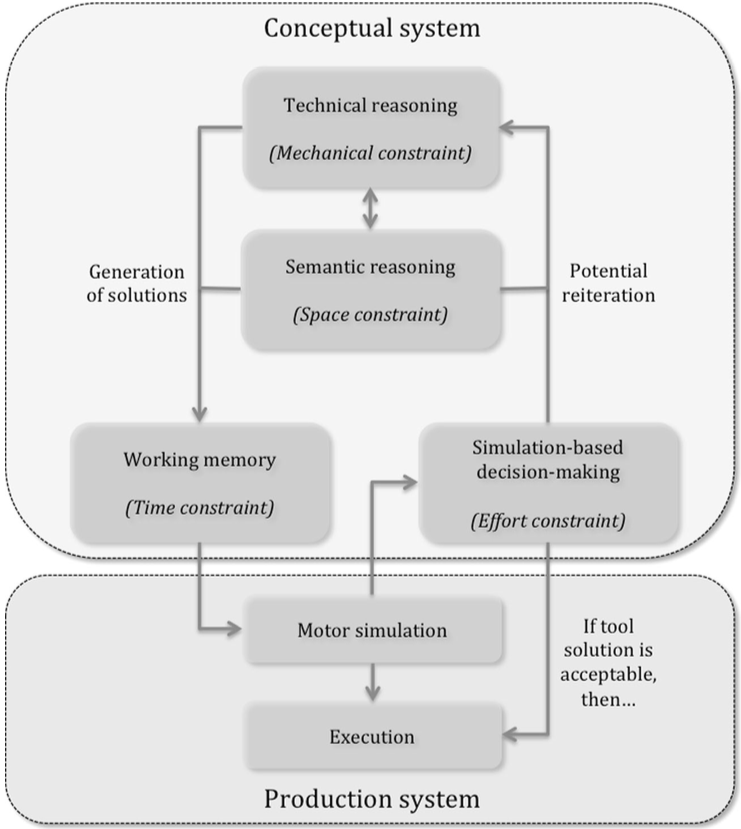
\includegraphics[width=0.9\textwidth]{4CTArchitecture.png}
	\caption{4CT Architecture\cite{osiurak2014}}
	\centering
	\label{fig:4CTArcithecture}
\end{figure}

\subsection{Mechanical Constraint}
In real world tool use, the fundamental challenge is how physical principles can transform the environment to the desired state. Aiding this process is mechanical and object based knowledge. Mechanical knowledge encompasses the technique of usage (e.g. cutting, hammering), whilst object based knowledge is represented by the tool's physical properties (e.g. hardness, length, weight). 

A tool is suitable to use with an object if their properties form a complementary fit (e.g. tool sharpness with object softness ). Technical reasoning is the cognitive enabler through which an individual is able to match tools and objects to bring the desired transformations. 4CT assumes that tools and objects are stored relative to each other based on such properties. The hypothesis offers some insight in representing object knowledge. 

Mechanical knowledge helps form representations of intended tool movement. The  production system later turns these intentions into actual body movement. The theory, however, does not describe this process. Techniques of usage usually have resulting forces or effects ( e.g. using an object as a lever generates a force on the opposite extreme) . 4CT focuses on physical attributes of objects (e.g abrasiveness, hardness) with no account for mechanical forces.

\pagebreak

\subsection{Space Constraint}
The space constraint is better explained and understood through the process that solves it, semantic reasoning. Objects and tools are semantically related through a form of categorisation (e.g. bread and knife are both kitchen items). Semantic reasoning helps determine and spatially locate the right tool and object based on their categorical relation (e.g. knife and bread are most likely in the kitchen ). In other words the space constraint optimises the search problem. This is in contrast to how technical reasoning associates the object and tool based on their physical properties.

\subsection{Time Constraint}
The time constraint is again best defined through the process that solves it, working memory. The time constraint represents the subject's ability to hold goals in working memory. In satisfying a higher level objective, a subject would split the task into intermediate steps and objectives. Being able to achieve these concomitantly is limited by memory storage. It is, however, unclear why this is considered to be time dependent instead of storage capacity dependent. 

\subsection{Effort Constraint}
In satisfying transformations of the environment we have to be aware of the energy costs associated. The effort constraint covers the costs of tool use. One of the rules of survival is that actions should be less expensive than the reward gained\cite{profet2006}. The cost of effort can help explore and select from the space of possible solutions. 

In a situation where using hands would be optimal, subjects still show a preference for using tools\cite{osiurak2014}. This demonstrates that humans usually overestimate the benefits gained and that effort measurement is not representative of the real energy cost. The measurement of effort is likely to be more speculative based on past experience. 

The theory considers costs to be estimated through a process of mental simulation. However, if simulation based decision making determines effort, it must have some level of sensorimotor information. This contradicts the previous statement that the conceptual level has no such knowledge.

\section{Limitations}
To summarise, 4CT focuses on the conceptual components of tool use. It assumes that use cases are problem situations\cite{osiurak2014}. The four constraints and their associated processes outline the components of tool use reasoning. The theory, however, does not go into detail. It is not explicit on how representations for mechanical and object knowledge are formed. We can assume that these emerge from experience through learning. However, without insight into this process the conceptual components may be constrained in ways we are not aware of.

Although not explicit, 4CT distinguishes between tools and objects they apply to. For example, technical reasoning is described as a single tool to object relation. This distinction is unrequited. In cases when appropriate tools are not available, objects can become novel tools.

It is difficult to envision how other tool use scenarios would be covered. Consider cases when multiple objects form the tool, such as a chisel and hammer. Alternatively, what happens when the tool acts directly on the environment, such as a shovel digging a hole. The theory's technical reasoning can not easily explain these cases, especially if the tool's purpose is to avoid environment obstacles ( e.g. an L shaped bar hooking an object from a cylinder).

As the details of technical reasoning and mental simulation are not fully described, a computational model will have to assume how tool technique manifests into physical principles and how effort is measured without sensorimotor information. 

Some of the theory's limitations are borne from it being exclusively developed on apraxia related investigations. It would have been interesting to also consider an evolutionary basis. Animal tool use literature is ample, with experiments similar to apraxia research. For example New Caledonian crows are able to fashion hooks out of straight wires in order to extract food from cylinders\cite{bettyCrow2009}. 

\section{Computational Model Importance}
The outlines defined by 4CT are simple and intuitive. However, missing aspects emerge when considering the implementation of a computational model. Even in a symbolic approach the construction of a model will highlight where the theory can be improved. 

Because technical reasoning is the most detailed part of the theory, it becomes a reasonable aspect to focus on. The model however will have to make assumptions outside of the theory in order to cover more convincing cases of tool use. 

\begin{thebibliography}{9}
\bibitem{osiurak2013}
Osiurak, F., Jarry, C., Lesourd, M., Baumard, J., \& Le Gall, D. (2013). \emph{Mechanical problem-solving strategies in left-brain damaged patients and apraxia of tool use}. Neuropsychologia, 51(10), 1964–1972.
doi:10.1016/j.neuropsychologia.2013.06.017

\bibitem{osiurak2014}
Osiurak, F. (2014). \emph{What Neuropsychology tells us about human tool use? The Four constraints theory (4CT): Mechanics, space, time, and effort}. Neuropsychology Review, 24(2), 115 - 88. doi:10.1007/s11065-014-9260-y


\bibitem{fitch2010}
Fitch, T. W. (2010). \emph{The evolution of language (4th ed.)}. Cambridge: Cambridge University Press.

\bibitem{oxford}
Tool (n.d.). In Oxford DictionaryOxford University Press. Retrieved from http://www.oxforddictionaries.com/definition/english/tool

\bibitem{bettyCrow2009}
Bird, C. D., \& Emery, N. J. (2009). \emph{Insightful problem solving and creative tool modification by captive nontool-using rooks}. Proceedings of the National Academy of Sciences, 106(25), 10370–10375. doi:10.1073/pnas.0901008106

\bibitem{profet2006}
Proffitt, D. R. (2006). \emph{Embodied perception and the economy of action}. Perspectives on Psychological Science, 1(2), 110–122. doi:10.1111/j.1745-6916.2006.00008.x

\end{thebibliography}

\end{document}